\pdfoutput=1
\documentclass[11pt]{article}
\usepackage[utf8]{inputenc}
\usepackage[T1]{fontenc}
\usepackage{amsmath,amssymb,amsthm}
\usepackage{graphicx}
\usepackage{tikz}
\usepackage{hyperref}
\usepackage{cleveref}
\newcommand{\method}{\textsc{AdaThresh}}
\newcommand{\R}{\mathbb{R}}
\DeclareMathOperator*{\argmin}{arg\,min}


\newtheorem{theorem}{Theorem}

\title{Sparse Feature Selection with Adaptive Thresholds}
\author{A. Author \and B. Author}

\begin{document}
\maketitle

\begin{abstract}
We study feature selection for linear regression when the number of features is large.
We propose \method{}, a simple procedure that adapts its threshold to the noise level,
and we show that it recovers the true support with high probability.
\end{abstract}

\section{Introduction}\label{sec:intro}
High-dimensional regression appears in many applications, such as genomics and signal processing.
The Lasso~\cite{tibshirani1996} is a popular estimator, but its performance may depend heavily on the choice of the regularization parameter.
In this paper, we propose a method that chooses this parameter from the data (\cref{sec:method}).

Our contributions are as follows.
\begin{itemize}
  \item We introduce \method{}, an adaptive thresholding rule.
  \item We prove that it recovers the support under mild conditions (Theorem~\ref{thm:main}).
\end{itemize}


\section{Method}\label{sec:method}
% This comment line is removed before translation.
Let $X \in \mathbb{R}^{n \times p}$ be the design matrix and $y$ the response.
Our estimator solves
\begin{equation}
  \hat{\beta} = \arg\min_{\beta} \frac{1}{2n}\|y - X\beta\|_2^2 + \lambda \|\beta\|_1 , \label{eq:lasso}
\end{equation}
where $\lambda$ is chosen adaptively, as summarized in \cref{fig:overview}.

\begin{theorem}[Support recovery]\label{thm:main}
Under the irrepresentable condition, \method{} recovers the support of $\beta^*$ with probability at least $1 - \delta$.
\end{theorem}

\begin{figure}[t]
  \centering
  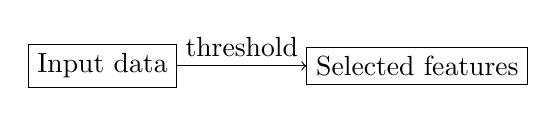
\begin{tikzpicture}
  \node[draw] (a) at (0,0) {Input data};
  \node[draw] (b) at (4,0) {Selected features};
  \draw[->] (a) -- node[above] {threshold} (b);
\end{tikzpicture}

  \caption{Overview of the proposed procedure. The text inside the figure is kept as is.}
  \label{fig:overview}
\end{figure}

The implementation is a single function call:
\begin{verbatim}
beta = adaptive_lasso(X, y)  # 100% vectorized
\end{verbatim}

\section{Experiments}
Table~\ref{tab:res} reports the support recovery rate on synthetic data.
\begin{table}[h]
  \centering
  \begin{tabular}{lcc}
    Method & Recall & Precision \\
    \hline
    Lasso & 0.81 & 0.74 \\
    \method & 0.93 & 0.90 \\
  \end{tabular}
  \caption{Support recovery on synthetic data.}
  \label{tab:res}
\end{table}

\bibliographystyle{plain}
\bibliography{refs}
\end{document}
